\section{Auswertung}
\label{sec:Auswertung}
\subsection{Strömungsgeschwindigkeit}
Die gemessenen Frequenzverschiebungen sind in Tabelle \ref{tab:Messwertedf} für alle 3 Prismawinkel mit ihren zugehörigen 
Dopplerwinkeln $\alpha$ und bei 5 verschiedenen Fließgeschwindigkeiten aufgetragen. Die Dopplerwinkel ergeben sich nach Formel\eqref{eq:alp}.
Die Messfrequenz der Ultraschallsonde beträgt $\nu_0=\qty{2}{\mega\Hz}$.
\begin{table}[H]
  \centering
  \caption{Gemessene Frequenzunterschiede für 5 verschiedene Fließgeschwindigkeiten und 3 verschiedene Prismawinkel.}
  \label{tab:Messwertedf}
  \begin{tabular}{S[table-format=2] S[table-format=2.2] S[table-format=3] S[table-format=3] S[table-format=3]S[table-format=3]S[table-format=4]}
      \toprule
      {$\theta$}&{$\alpha$}&{$\Delta \nu_{\qty{1.5}{\liter}}$/Hz}&{$\Delta \nu_{\qty{2.5}{\liter}}$/Hz}&{$\Delta \nu_{\qty{3.5}{\liter}}$/Hz}&{$\Delta \nu_{\qty{4.5}{\liter}}$/Hz}&{$\Delta \nu_{\qty{6}{\liter}}$}/Hz\\
      \midrule
      30 & 80,06 & 68 & 132 & 264 & 423 & 769 \\
      15 & 70,53 & 62 & 122 & 236 & 346 & 574 \\
      60 & 54,74 & 145 & 310 & 506 & 736 & 1182 \\
      \bottomrule
  \end{tabular}
\end{table}
\noindent Die Strömungsgeschwindigkeit berechnet sich nach Umstellen von Gleichung \eqref{eq:deltaf}. Die Geschwindigkeiten, die sich 
bei den variierenden Dopplerwinkeln und Fließgeschwindigkeiten ergeben, sind in Tabelle \ref{tab:v} aufgelistet. Nun wird die Dopplerverschiebung $\Delta \nu$
normiert auf den Kosinus des jeweiligen Dopplerwinkels $\alpha$ gegen die resultierenden Strömungsgeschwindigkeiten aufgetragen.
Die Ergebnisse für den Prismawinkel $\theta = 15°$ sind in Abbildung \ref{fig:v15}, die für $\theta = 30°$ in Abbildung \ref{fig:v30} und die für $\theta = 60°$ in Abbildung \ref{fig:v60} zu sehen.
\begin{table}[H]
  \centering
  \caption{Strömungsgeschwindigkeiten $v$ bei verschiedenen Fließgeschwindigkeiten $v_\text{Fl}$ und Prismawinkeln $\theta$.}
  \label{tab:v}
  \begin{tabular}{S[table-format=1.1] S[table-format=1.2] S[table-format=1.2] S[table-format=1.2]}
      \toprule
      {$v_\text{Fl}$}&{$v_\text{15°}$}&{$v_\text{30°}$}&{$v_\text{60°}$}\\
      \midrule
      1,5 & 0,16 & 0,09 & 0,11 \\
      2,5 & 0,32 & 0,18 & 0,24 \\
      3,5 & 0,62 & 0,36 & 0,39 \\
      4,5 & 0,90 & 0,57 & 0,57 \\
      6 & 1,50 & 1,04 & 0,92 \\
      \bottomrule
  \end{tabular}
\end{table}

\begin{figure}[H]
  \centering
  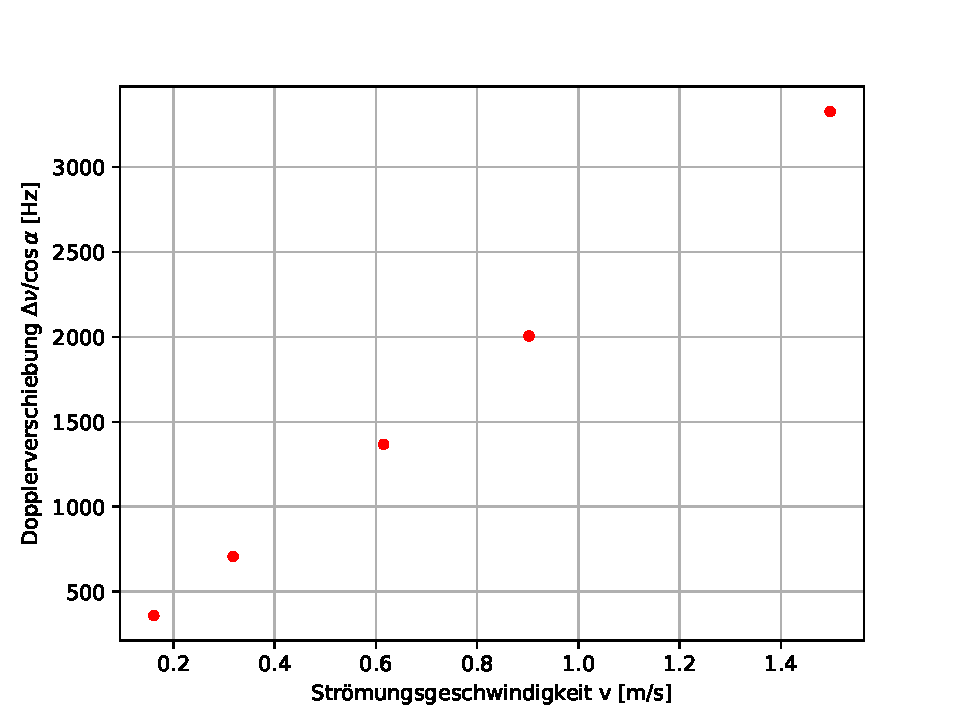
\includegraphics{build/Geschwindigkeit15.pdf}
  \caption{Dopplerverschiebung bei variierender Fließgeschwindigkeit gemessen bei $\theta=15°$.}
  \label{fig:v15}
\end{figure}

\begin{figure}[H]
  \centering
  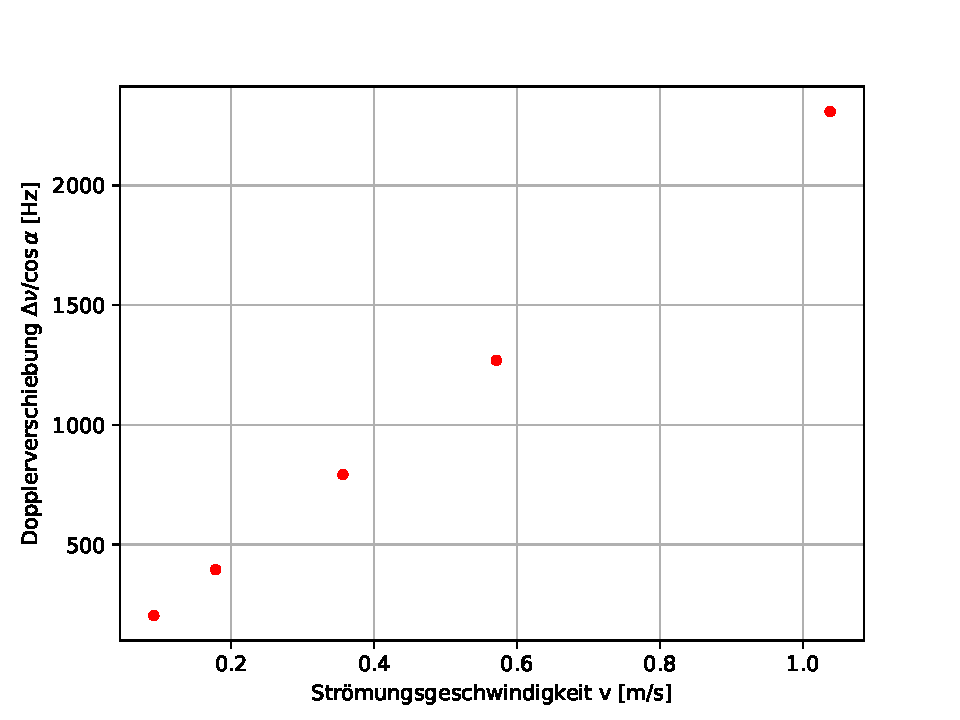
\includegraphics{build/Geschwindigkeit30.pdf}
  \caption{Dopplerverschiebung bei variierender Fließgeschwindigkeit gemessen bei $\theta=30°$.}
  \label{fig:v30}
\end{figure}

\begin{figure}[H]
  \centering
  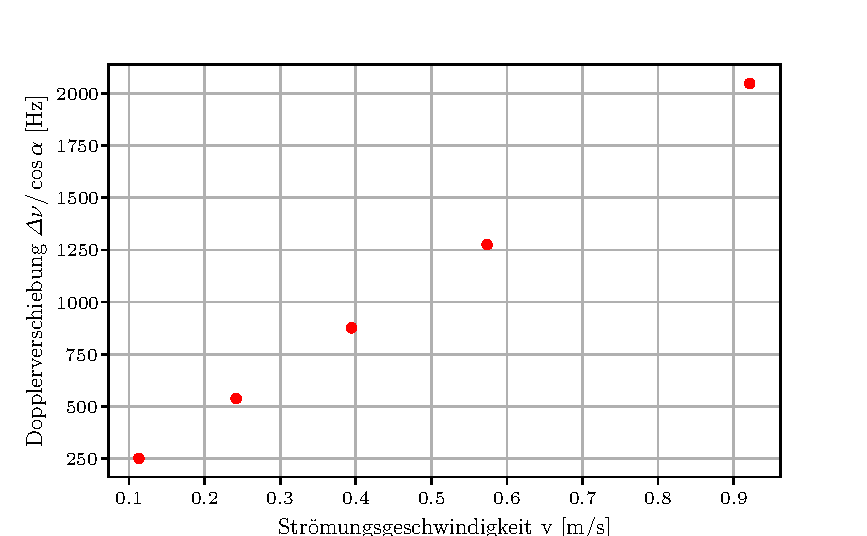
\includegraphics{build/Geschwindigkeit60.pdf}
  \caption{Dopplerverschiebung bei variierender Fließgeschwindigkeit gemessen bei $\theta=60°$.}
  \label{fig:v60}
\end{figure}

\subsection{Strömungsprofil}
Nun soll das Strömungsprofil des Innenrohrs untersucht werden. Dafür wird die Geschwindigkeit und 
die Streuintensität bei verschiedenen Messtiefen gemessen. Zur Besseren Vergleichbarkeit ist dies bei 2 verschiedenen 
Pumpleistungen durchgeführt worden. Die erste ist bei 40\% Pumpleistung durchgeführt worden, was $\qty{3.4}{\liter\per\minute}$ entspricht.
Die zweite wurde bei 70\% also $\qty{5.3}{\liter\per\minute}$ gemessen. Die Messergebnisse sind in Tabelle \ref{tab:Profil} aufgeführt.
Die Messtiefe ist am Messgerät als eine Absorptionszeit $t$ angegeben. Um nun die entsprechende Tiefe $s$ in mm zu bekommen, muss
die Zeit über die Schallgeschwindigkeit in eine entsprechende Strecke überführt werden. Dabei muss beachtet werden, dass die Materialien unterschiedliche
Schallgeschwindigkeiten besitzen und so die Umrechnung im Prisma sich von der in der Dopplerflüssigkeit unterscheidet. Der erste Messpunkt
bei $\qty{12}{\micro\second}$ ist so gewählt worden, dass er genau der Messtiefe von 30mm entspricht, was die genau dem Abstand zwischen Sonde
und Flüssigkeit entspricht. Die Umrechnung danach erfolgt über
\begin{equation}
  s=\frac{2}{3}\cdot t.
\end{equation}
Die Streuintensität und die Strömungsgeschwindigkeit sind für beide Pumpleistungen in Abbildung \ref{fig:si} und \ref{fig:sv} gegen die Messtiefe aufgetragen. 
\begin{table}[H]
  \centering
  \caption{Streuintensität und Strömungsgeschwindigkeit bei Messtiefen von 12$\unit{\micro\s}$ bis 20$\unit{\micro\s}$.}
  \label{tab:Profil}
  \begin{tabular}{S[table-format=2.1] S[table-format=4] S[table-format=2.1] S[table-format=4]S[table-format=3]S[table-format=2.1]}
      \toprule
      {Messtiefe/$\unit{\micro\s}$}&{Si$_\text{40\%}$/$\unit{m^2\per\second\cubed}$}&{v$_\text{40\%}$/$\unit{m\per\second}$}&{Si$_\text{70\%}$/$\unit{m^2per\second\cubed}$}&{v$_\text{70\%}$/$\unit{m\per\second}$}\\
      \midrule
      12 & 83 & 31,8 & 23 & 0 \\
      12,5 & 170 & 31,8 & 64 & 47,8 \\
      13 & 768 & 31,8 & 241 & 47,8 \\
      13,5 & 1065 & 34,5 & 412 & 55,7 \\
      14 & 1453 & 42,4 & 717 & 63,7 \\
      14,5 & 1536 & 47,8 & 801 & 76,9 \\
      15 & 1623 & 47,8 & 980 & 87,5 \\
      15,5 & 1481 & 45,1 & 894 & 95,5 \\
      16 & 1432 & 44,4 & 1068 & 103,5 \\
      16,5 & 1365 & 39,8 & 1103 & 103,5 \\
      17 & 1323 & 37,1 & 1152 & 90,2 \\
      17,5 & 1059 & 35,8 & 1010 & 84,9 \\
      18 & 857 & 34,5 & 1090 & 76,9 \\
      18,5 & 722 & 37,1 & 941 & 84,9 \\
      19 & 512 & 39,8 & 762 & 90,2 \\
      19,5 & 406 & 39,8 & 601 & 90,2 \\
      \bottomrule
  \end{tabular}
\end{table}

\begin{figure}[H]
  \centering
  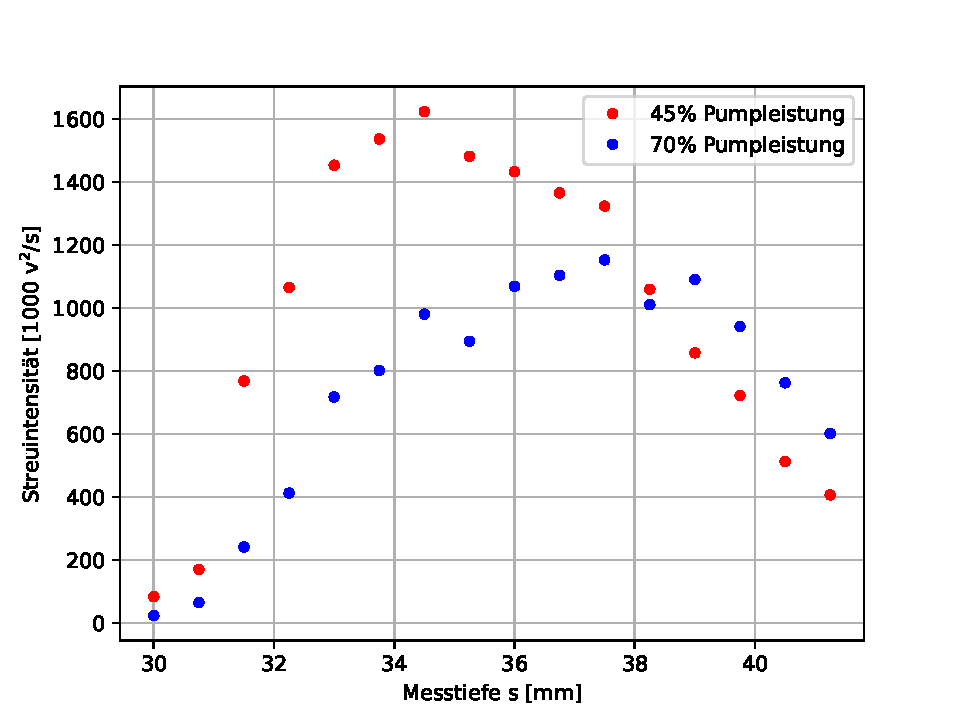
\includegraphics{build/Streui.pdf}
  \caption{Streuintensität bei variierender Messtiefe.}
  \label{fig:si}
\end{figure}

\begin{figure}[H]
  \centering
  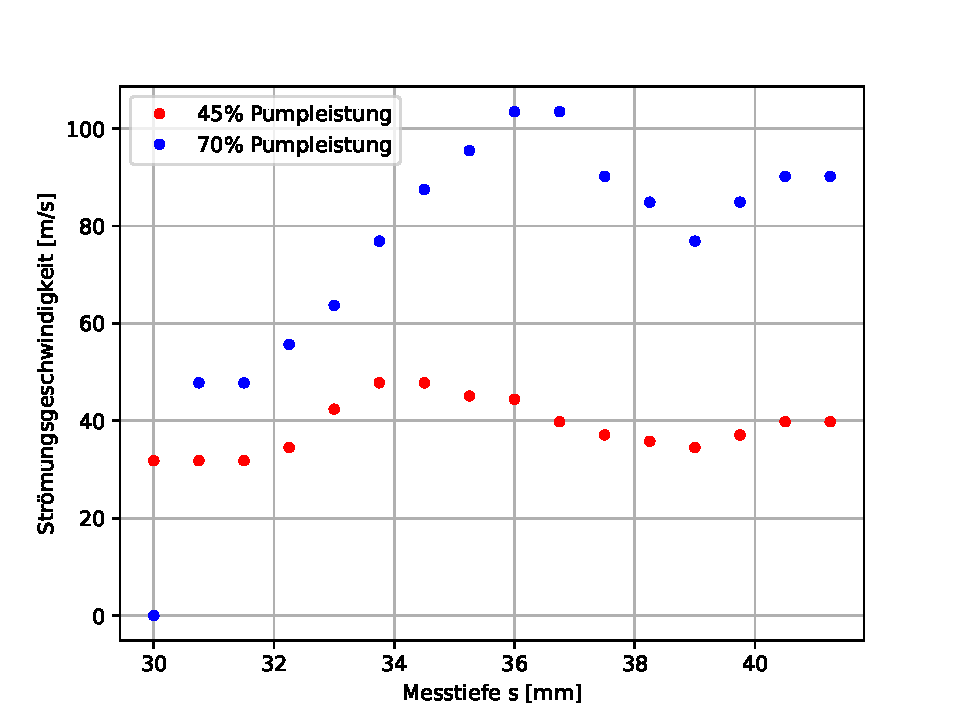
\includegraphics{build/Stroev.pdf}
  \caption{Strömungsgeschwindigkeit bei variierender Messtiefe.}
  \label{fig:sv}
\end{figure}
